\chapter{Grundlagen des Reinforcement Learning}\label{chap:grundlagen_rl}
Autonome Systeme bieten die Möglichkeit zur selbständigen Lösung komplexer oder für Menschen gefährlicher Probleme in potenziell unbekannten Umgebungen. 
Die technische Umsetzung dieser Systeme durch klassische Programmierparadigmen ist in vielerlei Hinsicht problematisch.
So ist der Zustandsraum in realen Anwendungen extrem groß. 
Insbesondere in fremden Umgebungen mangelt es klassischen Programmen an Allgemeingültigkeit. 
Das System sollte das Problem auch in unbekannten Umgebungen lösen können, ohne dass eine Anpassung der Logik notwendig ist.
Als zusätzliche Stufe der Komplexität ergibt sich zudem die Interaktion mit Menschen oder anderen autonomen Systemen. 
\ab
Menschen lernen von früh auf, indem sie den Einfluss ihrer Aktionen auf die Umgebung \cite[S. 1]{sutton2018} beobachten und daraus Schlüsse ziehen.
Jede Reaktion der Umwelt auf das Verhalten wird verarbeitet und beeinflusst die spätere Wahl der Aktionen.
Der Mensch entwickelt sich dadurch im Laufe der Zeit \cite[S. 634]{castano}.
Formal sind viele Reinforcement-Learning-Verfahren angelehnt an das psychologische Phänomen der operanten Konditionierung \cite[S. 34]{lefrancois1986}. 
Laut Skinner wird operante Konditionierung folgendermaßen beschrieben: 
\enquote{Wenn eine Reaktion [...] von einer Verstärkung gefolgt wird, so resultiert daraus eine Erhöhung der Wahrscheinlichkeit, dass diese Reaktion später unter ähnlichen Umständen wieder auftritt.}\cite[34]{lefrancois1986}.
Analog dazu sinkt die Wahrscheinlichkeit, wenn die Aktion bestraft wird.
Das Ausprobieren von Aktionen erfolgt nach dem Versuchs- und Irrtums-Prinzip \cite[S. 2f]{sutton2018}.
Die Schwierigkeit dabei ist, dass die Aktionen nicht nur Einfluss auf den direkten Folgezustand, sondern auch nachhaltig auf spätere Zustände nehmen.
So kann die vermeintlich optimale Aktion zwar kurzfristig die Belohnung maximieren, langfristig aber nicht optimal sein.
Der Agent muss dabei abwägen, ob bestehendes Wissen genutzt wird (engl. exploitation) oder neues Wissen hinzugewonnen werden soll (engl. exploration).
\ab
Anders als bei anderen maschinellen Lernverfahren, wie beim überwachten Lernen, ist das Ziel des Reinforcement Learning nicht, Wissen aus vorher manuell bewerteten Informationen, sondern aus Aktionen und dessen Auswirkung zu generalisieren.
Überwachte Lernverfahren sind in vielen Domänen sinnvoll und können gute Lösungen hervorbringen.
Durch die vom Menschen benötigten Information über die Klassenzugehörigkeit der Daten ist dieser Ansatz jedoch nur beschränkt für komplexe Umgebungen anwendbar.
\ab
Reinforcement Learning ist nicht ein einzelner Algorithmus, sondern ein Paradigma des maschinellen Lernens, welches aus einer Sammlung von Algorithmen und Vorangehensweisen zusammengesetzt ist.
Deshalb wird im Folgenden das Konzept des Markov-Entscheidungsprozesses als Grundlage des Reinforcement Learning beschrieben. 
Zusätzlich werden Eigenschaften von Reinforcement-Learning-Verfahren aufgezeigt, um daraus in der späteren Konzeption \autoref{sec:massnahmen} technische Maßnahmen ableiten zu können.

\section{Markov-Entscheidungsprozess}\label{sec:markov}
Allgemein können Reinforcement-Learning-Probleme mit Hilfe eines Markov"=Entscheidungsprozesses (engl. Markov decision process) \cite[S. 636]{castano} formalisiert werden.

\begin{figure}
    \centering
    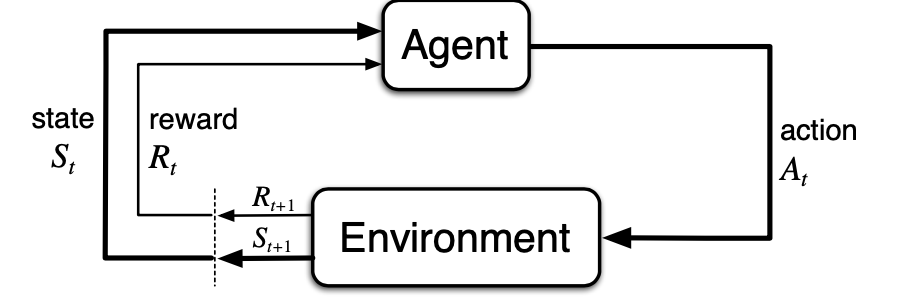
\includegraphics[width=1.0\textwidth]{graphics/markov.png}
    \caption{Ablauf des Markov-Entscheidungsprozess}
    \label{fig:markov_ablauf}
\end{figure}

Der Ablauf wird in \autoref{fig:markov_ablauf} dargestellt und kann laut \cite[S. 636]{castano} als ein \enquote{[...]discrete state-time transition system [...]} beschrieben werden. 
Die zwei Hauptbeteiligten Objekte sind Agent und Umwelt \cite[S. 47ff.]{sutton2018}.
Ein Agent beschreibt eine mit seiner Umwelt interagierende Entität und kann über Software oder Hardware abgebildet werden.
Alle Variablen sind abhängig von diskretisierten Zeitpunkten $t$.
Der Agent erhält zu jedem Zeitpunkt den aktuellen Zustand (engl. state) $s$.
Er kann dann mit der Umwelt z.B. durch Aktoren interagieren, indem er eine Aktion (engl. action) $a \in A_t$ ausführt, wobei die Menge $A_t$ alle Aktionen, die der Agent zum Zeitpunkt $t$ ausführen kann, beschreibt.
Die Wahrscheinlichkeit für den Übergang in den Folgezustand $S_{t+1}$ wird beschrieben durch die Verhaltensstrategie $\pi(a|s_t)$ \cite[S. 58]{sutton2018}.
Für jedes Zustands-Aktions-Paar wird durch eine Belohnungsfunktion eine Belohnung $r_t(s_t, a_t)$ berechnet \cite[S. 638]{castano}.
Ziel ist eine möglichst optimale Abfolge von Aktionen zu ermitteln, um die Summe der Belohnungen zu maximieren.

\section{Begriffe und Eigenschaften von Reinforcement Learning Verfahren}\label{sec:eigenschaften_rl}
Dadurch, dass Reinforcement Learning nicht einen einzelnen Algorithmus beschreibt, sondern ein Paradigma bestehend aus einer Vielzahl von Algorithmen, ist es im Hinblick auf das Ziel dieser Arbeit sinnvoll, die unterscheidenden Merkmale der Verfahren zu betrachten.
Die Begriffe werden als Entscheidungskriterien in \autoref{sec:massnahmen} hinzugezogen, sodass insbesondere im Hinblick auf die Kompabilität mit den in \autoref{sec:def_ethischer_werte} definierten Werten die Wahl eines geeigneten Verfahrens vereinfacht werden kann.
\subsection{Belohnung und Wertfunktion}
Als Reaktion der Umwelt auf eine Aktion des Agenten wird durch eine stochatische Funktion \cite[S. 6]{sutton2018} eine Belohnung zurückgeliefert.
Die Belohnung ist die Grundlage für eine meist unverzügliche Anpassung der Verhaltensstrategie und dient als Indikator über die Güte der ausgeführten Aktion für den jeweiligen Zustand.
Um nachhaltig sinnvolle Entscheidungen zu treffen existiert zusätzlich die Wertfunktion (engl. value function), welche den langfristigen Nutzen von Zuständen approximiert.
So kann beispielsweise ein Zustand einzeln betrachtet stets in einer geringen Belohnung resultieren, langfristig jedoch von gut belohnten Zuständen gefolgt sein.
Die Wertfunktion ordnet diesem Zustand einen hohen Wert zu, die Belohnungsfunktion hingegen einen niedrigen Belohnungswert.

\subsection{Model-freie und Model-basierte Verfahren}
Im Kontext der model-freien und der model-basierten Verfahren bezeichnet das Model die Kenntnis einer Abbildung der Umwelt und dessen Verhalten \cite[S. 7]{sutton2018}.
Das Model der Umwelt wird abgebildet durch eine Zustandsübergangsfunktion \cite[S. 14]{li2018}.
Wird ein model-basiertes Verfahren genutzt, so existiert ein solches Model über die Umwelt und kann genutzt werden, um Vorhersagen über die Auswirkungen von Aktionen zu treffen.
Existiert kein Model muss ein model-freies Verfahren benutzt werden.
Mit Hilfe des Versuchs- und Irrtumsprinzip \cite[S. 7]{sutton2018} versucht der Agent dann, je nach Verfahren ein eigenes Model der Umwelt zu erzeugen.

\subsection{On-Policy und Off-Policy}
On-Policy und Off-Policy beschreiben Lernverfahren, die sich insbesondere durch das Vorgehen bezüglich der Verwendung und Anpassung der Verhaltensstrategie bzw. im Fall des Off-Policy Lernens der Zielstrategie unterscheiden.
Beim Off-Policy Lernen \cite[S. 14]{li2018} wird eine meist statische Vorgehensstrategie (engl. behavior policy) benutzt, welche das Verhalten des Agenten steuert. 
Zusätzlich gibt es eine Zielstrategie (engl. target policy), welche eine möglichst optimale Wertfunktion lernt.
Die Zielstrategie wird basierend auf den erhaltenen Belohnungen für die ausgeführten Aktionen angepasst.
On-Policy-Lernen benutzt nur eine einzelne Verhaltensstrategie, welche ähnlich wie die Zielstrategie des Off-Policy-Lernens angepasst wird, jedoch auch zur Steuerung des Verhaltens des Agenten benutzt wird.